% do not change these two lines (this is a hard requirement
% there is one exception: you might replace oneside by twoside in case you deliver 
% the printed version in the accordant format
\documentclass[11pt,titlepage,oneside,openany]{book}
\usepackage{times}


\usepackage{graphicx}
\usepackage{latexsym}
\usepackage{amsmath}
\usepackage{amssymb}
\usepackage{subfigure}

\usepackage{ntheorem}

% \usepackage{paralist}
\usepackage{tabularx}

% this packaes are useful for nice algorithms
\usepackage{algorithm}
\usepackage{algorithmic}

% well, when your work is concerned with definitions, proposition and so on, we suggest this
% feel free to add Corrolary, Theorem or whatever you need
\newtheorem{definition}{Definition}
\newtheorem{proposition}{Proposition}


% its always useful to have some shortcuts (some are specific for algorithms
% if you do not like your formating you can change it here (instead of scanning through the whole text)
\renewcommand{\algorithmiccomment}[1]{\ensuremath{\rhd} \textit{#1}}
\def\MYCALL#1#2{{\small\textsc{#1}}(\textup{#2})}
\def\MYSET#1{\scshape{#1}}
\def\MYAND{\textbf{ and }}
\def\MYOR{\textbf{ or }}
\def\MYNOT{\textbf{ not }}
\def\MYTHROW{\textbf{ throw }}
\def\MYBREAK{\textbf{break }}
\def\MYEXCEPT#1{\scshape{#1}}
\def\MYTO{\textbf{ to }}
\def\MYNIL{\textsc{Nil}}
\def\MYUNKNOWN{ unknown }
% simple stuff (not all of this is used in this examples thesis
\def\INT{{\mathcal I}} % interpretation
\def\ONT{{\mathcal O}} % ontology
\def\SEM{{\mathcal S}} % alignment semantic
\def\ALI{{\mathcal A}} % alignment
\def\USE{{\mathcal U}} % set of unsatisfiable entities
\def\CON{{\mathcal C}} % conflict set
\def\DIA{\Delta} % diagnosis
% mups and mips
\def\MUP{{\mathcal M}} % ontology
\def\MIP{{\mathcal M}} % ontology
% distributed and local entities
\newcommand{\cc}[2]{\mathit{#1}\hspace{-1pt} \# \hspace{-1pt} \mathit{#2}}
\newcommand{\cx}[1]{\mathit{#1}}
% complex stuff
\def\MER#1#2#3#4{#1 \cup_{#3}^{#2} #4} % merged ontology
\def\MUPALL#1#2#3#4#5{\textit{MUPS}_{#1}\left(#2, #3, #4, #5\right)} % the set of all mups for some concept
\def\MIPALL#1#2{\textit{MIPS}_{#1}\left(#2\right)} % the set of all mips





\begin{document}

\pagenumbering{roman}
% lets go for the title page, something like this should be okay
\begin{titlepage}
	\vspace*{2cm}
  \begin{center}
   {\Large The Extremes of Good and Evil\\}
   \vspace{2cm} 
   {Bachelor Thesis\\}
   \vspace{2cm}
   {presented by\\
    Larissa Strauch \\
    Matriculation Number 1518629\\
   }
   \vspace{1cm} 
   {submitted to the\\
    Data and Web Science Group\\
    Prof.\ Dr.\ Ponzetto\\
    University of Mannheim\\} \vspace{2cm}
   {August 2014}
  \end{center}
\end{titlepage} 

% no lets make some add some table of contents
\tableofcontents
\newpage

\listofalgorithms

\listoffigures

\listoftables

% evntuelly you might add something like this
% \listtheorems{definition}
% \listtheorems{proposition}

\newpage


% okay, start new numbering ... here is where it really starts
\pagenumbering{arabic}

\chapter{Introduction}

\section{Problem Statement}
 
 

\section{Contribution}

 

\section{Related Work}


\chapter{Data Analysis}
\label{cha:theory}


\section{Data Description}
 The given data, on which we want to build our model on, was provided by zenodo.org as part of SemEvals Task 4 and consists of 2 independent datasets, which in turn have been divided into a GroundTruth-, Training- and Validation set.
 
 \noindent The first dataset, recognizable by the term 'byPublisher', reflects the publisher's general bias set forth by BuzzFeed journalists or MediaBiasFastCheck.com beforehand. It consists of a total of 750,000 items, of which 600,000 belong to the Training- and 150,000 to the Validation set.
 
 \noindent In return, the second dataset, recognizable by the term 'byArticle', was scrapped by crowdsourcing at hand and therefore consists of only 645 items without a Validation set.\\
 \\
 The GroundTruth dataset was provided as an XML File and consists of the features 'article url', 'labeled-by', 'id' and 'hyperpartisan'. In addition, the GroundTruth dataset scrapped 'byPublisher' contains the feature 'bias'.
\begin{itemize}
	\item Article-url: Contains the article's url.
	\item Labeled-by: Reflects whether the respective article was labeled 'byPublisher' or 'byArticle'.
	\item Id: Allocates each article a unique id.
	\item Hyperpartisan: Displays whether the particular article has been labeled as hyperpartisan or not.
	\item Bias: Divides the publisher's bias into 'left', 'left-center', 'least', 'right-center' and 'right'.
\end{itemize}
 The Training dataset was as well provided as an XML file and contains the contents of the website of the respective article. In addition, it consists of the features 'article title' 'published-at' and 'id'.
\begin{itemize}
	\item Article title: Represents the articles title.
	\item Published-at: Specifies the published date.
	\item Id: A unique id, which is the same as the corresponding entry in the GroundTruth dataset.
\end{itemize}

 \noindent The given Data has been cleaned in advance, therefore no additional steps were necessary.\\ 
 The main focus of the datasets is on the Hyperpartisan feature, on which we want to classify the articles as this thesis progresses.
 

\subsection{Dataset labelled by Publisher}
As mentioned above, this dataset consists of a total of 750,000 articles and is divided into a training record consisting of 600,000 articles and a validation set consisting of 150,000 articles. Summarizing these two sets of data, a total of 375,000 were labelled as 'Hyperpartisan' and 375,000 were not – which corresponds to a 50:50 distribution. But even individually, this distribution does not change. 
\begin{figure}[h]
	\centering
	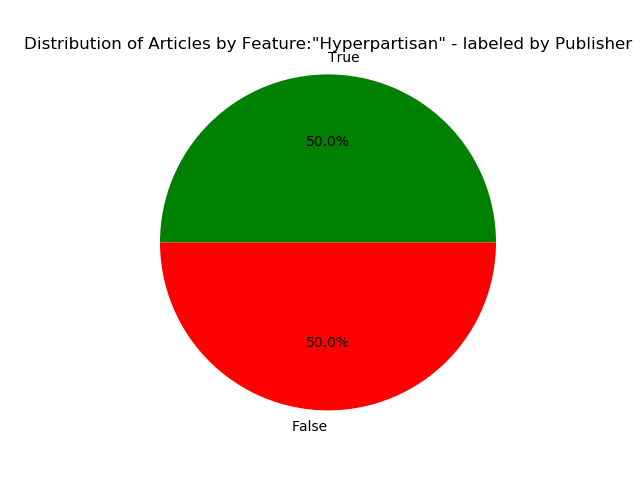
\includegraphics[width=0.5\textwidth]{C:/Users/Laris/Documents/Bachelorarbeit/Hypeprartisan_LabeledByPublisher.png}
	\caption{Distribution of as Hyperpartisan labelled articles by publisher}
	\label{fig:example}
\end{figure}

\noindent This dataset also includes the feature 'bias', which informs you about the general bias of the publisher. All 375,000 Hyperpartisan labelled all are assigned to either the left or right sectors, but none are right-centre, least or left-centre and are again 50:50 distributed.


\noindent The other 50\% are split between the remaining bias, with 'Least' owning the largest share at 37\%.\\
The publicity data is distributed over the years 1964-2018, with most of the data coming from 2012-2018.
\begin{figure}[h]
	\subfigure[Distribution of Bias]{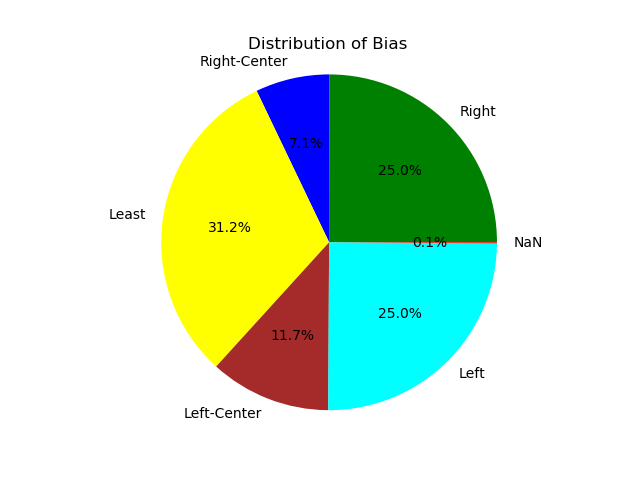
\includegraphics[width=0.5\textwidth]{C:/Users/Laris/Documents/Bachelorarbeit/Bias_Distribution.png}} 
	\subfigure[Distribution of publishing years]{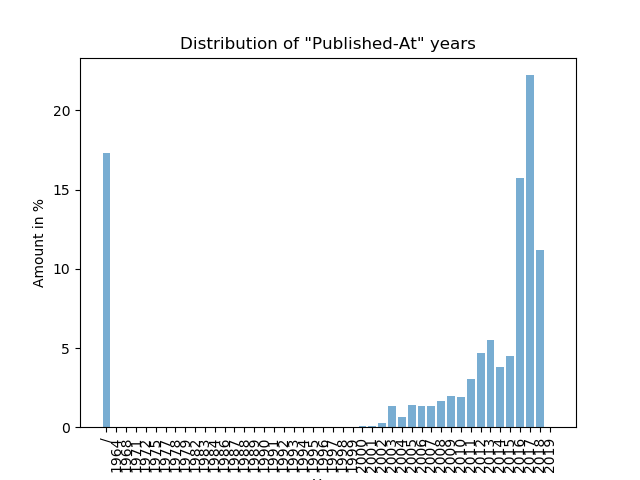
\includegraphics[width=0.5\textwidth]{C:/Users/Laris/Documents/Bachelorarbeit/Distribution_PublishedAt_Publisher_AllYears.png}} 
\end{figure}


\subsection{Dataset labelled by Article}

The dataset labelled by Article is a little different to the larger one labelled by publisher. Here the articles were individually labelled by hand. Accordingly, the distributions of this dataset are completely different. This becomes quiet obvious if we look at how the distribution of the Hyperpartisan labelled articles is here.
\begin{figure}[h]
	\subfigure[Distribution of Hyperpartisan labelled articles]{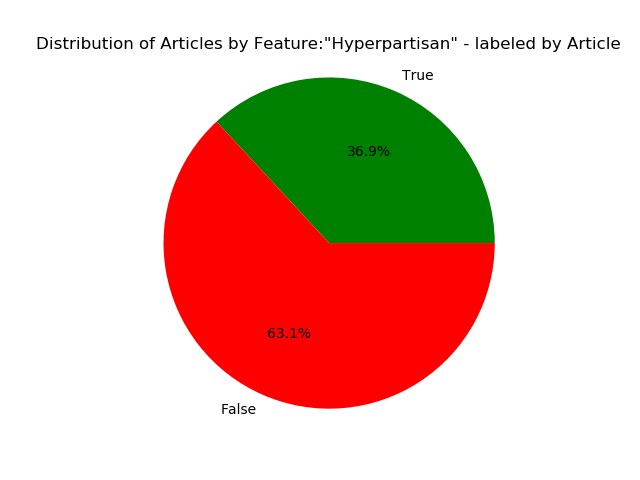
\includegraphics[width=0.5\textwidth]{C:/Users/Laris/Documents/Bachelorarbeit/Hypeprartisan_LabeledByArticle.png}} 
	\subfigure[Distribution of publishing years]{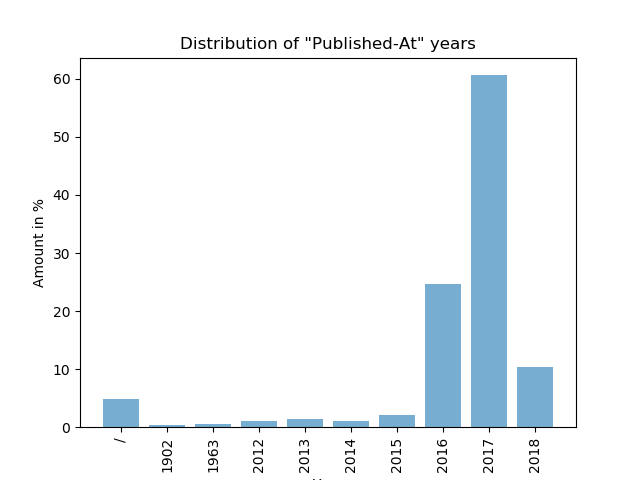
\includegraphics[width=0.5\textwidth]{C:/Users/Laris/Documents/Bachelorarbeit/Distribution_PublishedAt_Article}} 
\end{figure}
\noindent Here we can see that there is no 50:50 distribution left. Only 36.9\% were defined here as Hyperpartisan as shown in figure 2.4.\\
\noindent Moreover, in this dataset, the distribution of publication data is not mainly from the years 2012-2018, but in 2016-2018, with the largest number of articles dating back to 2017 at just under 60\% as we can see in figure 2.5. Altogether all 645 articles date from the years 1902-2018.

\section{Data Analysis}

Hyperpartisan means "extremely partisan; extremely biased in favor of a political party." [definition]. This often materializes in relation to significant political events. In the following chapter, I'll go into more detail about the direct link between the various features, especially the correlations between publication dates and label, as well as the connections between publisher and label.

  





\newpage


\pagestyle{empty}


\section*{Ehrenw\"ortliche Erkl\"arung}
Ich versichere, dass ich die beiliegende Master-/Bachelorarbeit ohne Hilfe Dritter
und ohne Benutzung anderer als der angegebenen Quellen und Hilfsmittel
angefertigt und die den benutzten Quellen w\"ortlich oder inhaltlich
entnommenen Stellen als solche kenntlich gemacht habe. Diese Arbeit
hat in gleicher oder \"ahnlicher Form noch keiner Pr\"ufungsbeh\"orde
vorgelegen. Ich bin mir bewusst, dass eine falsche Er- kl\"arung rechtliche Folgen haben
wird.
\\
\\

\noindent
Mannheim, den 31.08.2014 \hspace{4cm} Unterschrift

\end{document}
